Tras estudiar ardúamente el comportamiento de los distintos algoritmos desarrollados en el trabajo presente, se procedió a evaluarlos comparativamente todos sobre un nuevo conjunto de instancias del tipo \texttt{mágico}, con las siguientes decisiones:
\begin{itemize}
    \item Heurística golosa \texttt{Greedy} como unión de las heurísticas \texttt{GreedyA}, \texttt{GreedyB}, \texttt{GreedyC} 
    \item Metaheurística GRASP con los siguientes parámetros:
        \begin{itemize}
            \item Restricted Candidate List con $\beta = 10$
            \item Condición de terminación con 
            \begin{itemize}
                \item Máx. cantidad de iteraciones sin encontras solución inicial factible = $n^4$
                \item Máx. cantidad de iteraciones sin mejoras = $n^4$
                \item Máx. cantidad de iteraciones totales = $n^2$
            \end{itemize}
        \end{itemize}
\end{itemize}

\begin{figure}[H]
\begin{center}
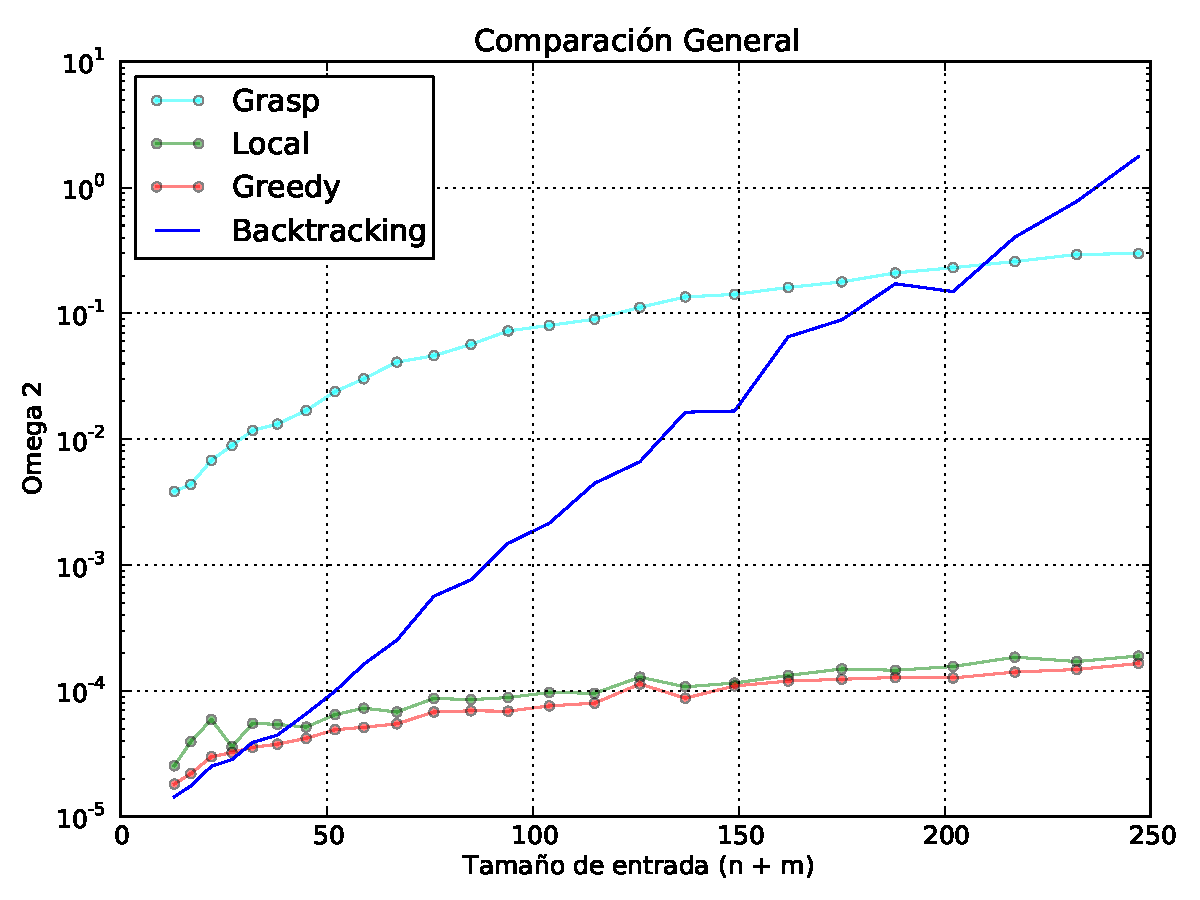
\includegraphics[angle=0, scale=.75]{imagenes/todas-tiempo.pdf}
\label{grafico local tiempo}
\caption{Tiempo de ejecución de los distintos algoritmos en nuevas instancias \textit{mágicas} de densidad media}
\end{center}
\end{figure}

Primero se evaluó el tiempo de ejecución en entradas chicas en las que \texttt{Backtracking} es todavía razonable en cuanto al tiempo de ejecución. En el gráfico se utilizó una escala logarítmica para observar con detalle las cuatro curvas, ya que en su defecto los tiempos de ejecución de \texttt{Greedy} y \texttt{Local} resultaban imperceptibles. Para tamaños de grafo menores a 50, \texttt{Grasp} presenta un tiempo de ejecución casi tes órdenes de magnitud por encima del resto de los algoritmos. Ésto se debe a la considerable cantidad de iteraciones que se le está permitido efectuar antes de retornar la mejor solución encontrada.

Por otra parte es notable la evolución del tiempo de ejecución de \texttt{Backtracking}. Comienza siendo el algoritmo más rápido, con una baja constante comparado con los otros algoritmos más sofisticados. Sin embargo, la cualidad factorial de su complejidad lo hace sobrepasar ampliamente a los otros algoritmos a medida que el tamaño del grafo aumenta.

Los tiempos de ejecución de \texttt{Greedy} y \texttt{local} presentan un desarrollo muy similar, manteniendo valores muy por debajo a los demás algoritmos. Especialmente en tamaños de grafo de tamaño reducido, \texttt{Local}, tras obtener la solución inicial mediante \texttt{Greedy}, no logra hacer muchas mejoras, por su tiempo de ejecución está muy ligeramente por encima del correspondiente a \texttt{Greedy}.

Luego se procedió a examinar la calidad de las soluciones obtenidas por las distintas heurísticas, siempre teniendo como parámetro la solución óptima encontrada por \texttt{backtrack}. Se utilizaron las mismas instancias generadas para estudiar los tiempos de ejecución en la sección anterior.

\begin{figure}[H]
\begin{center}
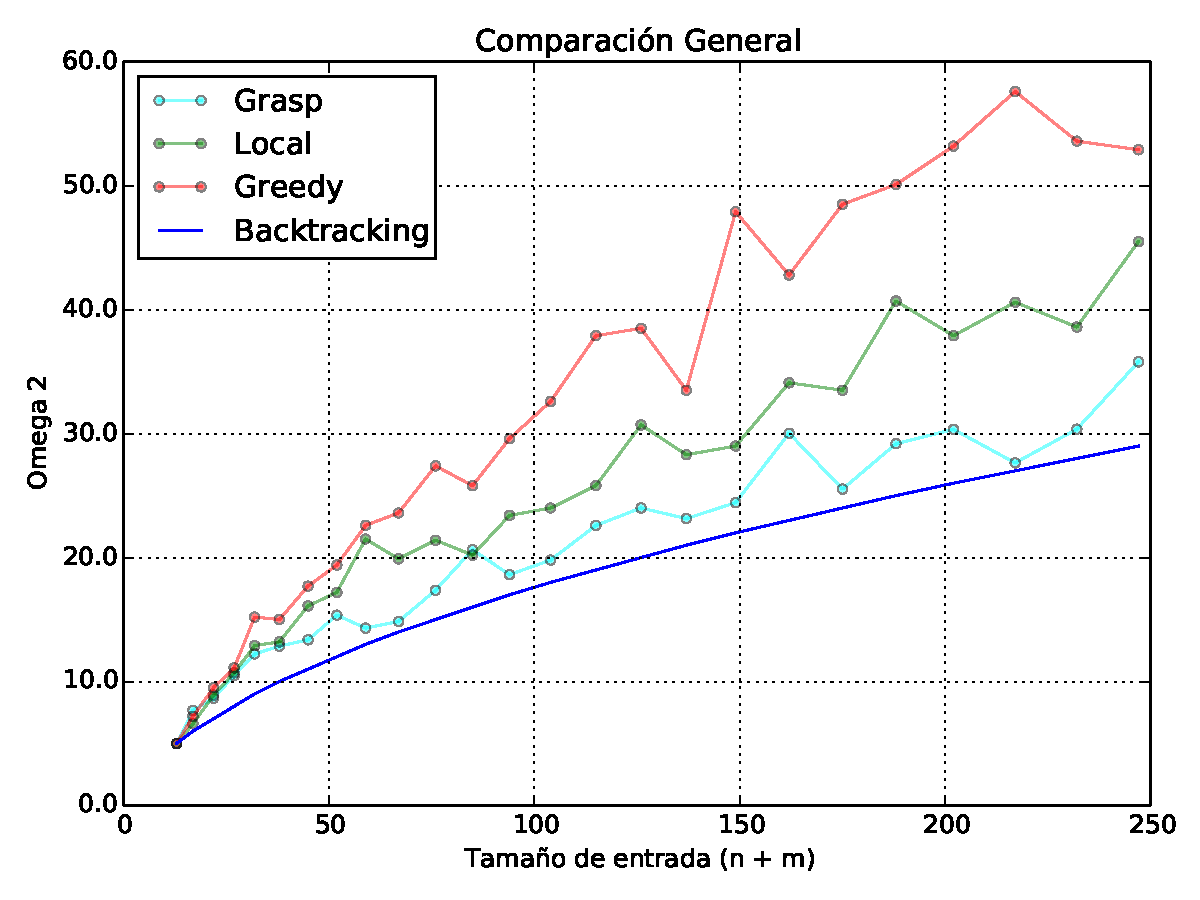
\includegraphics[angle=0, scale=.75]{imagenes/todas-calidad.pdf}
\label{grafico local calidad}
\caption{Calidad de solución de los distintos algoritmos en nuevas instancias \textit{mágicas} de densidad media}
\end{center}
\end{figure}

La solución encontrada por \texttt{Greedy}, en éstos tamaños de entrada, parece tener un $\omega_2$ acotado por el doble del $\omega_2$ de la solución óptima. Sin embargo, por lo que se puede llegar a percibir en las instancias de este tamaño, cabe la posibilidad de que su $\omega_2$ esté en realidad divergiendo del óptimo.

La solución encontrada por \texttt{Local} tiene un $\omega_2$ claramente por debajo de la solución encontrada por \texttt{Greedy}. A pesar de tener un tiempo de ejecución muy poco por encima de \texttt{Greedy}, logra un solución mucho más cercana a la óptima. Parece mantener cierta distancia relativa a la solución encontrada por \texttt{backtracking}.

La performace de \texttt{Grasp} merece consideración. Como invariante frente a los distintos tamaños de grafo, devuelve una solución bastante cerca de la óptima. Aunque para estos tamaños de grafo, el $overhead$ de la constante hace a \texttt{backtracking} quizás una alternativa más rápida.


\fixme{lo siguiente iria como en una sección de conclusion}
 
Asumimos trivialmente que el backtracking es el algoritmo que logra una mejor \textbf{calidad} al momento de obtener la solución, característica que sólo puede ser contrastada frente al inmenso tiempo que el mismo demora en correr. Resulta también interesante observar el comportamiento del \textbf{algoritmo goloso}, el cual presenta ejecuciones relativamente buenas, mientras que otras ejecuciones directamente no encuentran el algoritmo (se pasan del K); para poder representar este fenómeno se las representó por debajo del algoritmo exacto, de forma tal que se entiende que en las instancias en que el local arrojó un valor menor al backtracking, es porque la solución obtenida no era factible. Por otra parte, el tiempo de esta heurística es mínimo frente a todo el resto de los algoritmos, representando una buena opción para realizar un ``acercamiento rápido'' o ``estimación'' a la solución, ya sea obteniendo una válida o inválida. Aun así, también es necesario destacar que así como muchas de las instancias obtenidas son ``buenas'' desde cierto punto de vista, es notable el hecho de que muchas veces los resultados obtenidos son, aunque factibles, extremadamente malos en relación a la solución exacta. Esto último nos permite inferir que este tipo de heurísticas no nos permiten realizar una estimación ``segura'' sobre la factibilidad o calidad del resultado obtenido, siendo su resultado más bien una especie de ``tiro de ruleta''. Finalmente podemos observar a las heurísticas locales y GRASP, las cuales presentan soluciones en común, dado que GRASP es básicamente una ``aplicación iterativa'' de la local, combinada con un factor de aleatoriedad y ciertos criterios de terminación. Así, el resultado no nos sorprende al mostrarnos lo que de cierta forma ya esperabamos, la heurística de GRASP se comporta siempre ``mejor o igual'' que la local, es decir, existen instancias en que gracias a la aplicación de la aletoriedad en el goloso inicial, y debido a la iteració, se logra una mejoría notable de la calidad de la solución. Por otro lado, aunque GRASP presenta la desventaja de tener un costo tempral mayor a la local, luego de realizar un correcto \textbf{tuneo} de los criterios de finalización logramos establecer una buena relación tiempo/calidad.
